\newpage
\section{Exercise Block 1}
\label{sec:exercise-block-1}

\subsection{Exclusive OR (15min)}\label{subsec:ex-1}
\textbf{Construct an XOR gate using only the giant NAND gates.}

 XOR stands for exclusive OR. As the name suggest, it is very similar to the OR gate, except that it does not yield one when both inputs are one. In different words this means that the XOR is true whenever the two inputs are not equal. Follow the steps below to construct the XOR circuit.
\begin{enumerate}
	\item Write down the truth table.
	\item\label{it:1} Construct the disjunctive normal form from your truth table.
	\item Draw the circuit according to step \ref{it:1}.
	\item Transform the circuit in such a way that it only uses NAND Gates.
	\item Build the XOR you have drawn with the giant NAND gates.
	\item How many NAND gates do you need? See if you can loose one or two gates.
\end{enumerate}

\subsection{XOR to the Next (15min)}
\textbf{Construct the same XOR gate as in exercise \ref{subsec:ex-1} but this time with the breadboard using the tiny gates.}


\section{Excercise Block 2a}

\subsection{Half-Adder (30min)}
\subsubsection{Part 1}
A half-adder takes two bits $a$ and $b$ and adds them. It is called half-adder because two of them are needed in order to construct an adder which is able to add several bits. We will see later why this is the case.

Let's first look at the addition of two decimal digits. 

\begin{figure}[h]
	\centering		  
	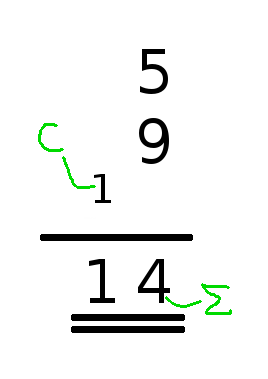
\includegraphics[scale=0.3]{decimal_addition.png}
	\caption{Decimal addition.}
	\label{fig:decimal_addition}
\end{figure}
We see that we need two things:
\begin{itemize}
	\item We need to know in which number the combination of 5 and 9 results. Namely 4.
	\item We need to carry a digit 1 because $5+9$ exceeds 10.
\end{itemize}

For binary digits (bits) we can do the same thing. Let's assume the following case. We have two 1 digit binary numbers. We call the single bit of the first number $a$ and the single bit of the second number $b$.
\begin{itemize}
	\item Write down all possible combinations of $a$ and $b$ in table \ref{tab:half-adder-truth-table}.
	\item Think about the output of each combination of $a$ and $b$ and write it into table \ref{tab:half-adder-truth-table} in the column $\Sigma$ (for sum). Which logical circuit does this resemble?
	\item Similar to the decimal case, we need to sometimes carry a bit. Write the value of the carry bit $c$ into table \ref{tab:half-adder-truth-table}. Now look at the columns $a$, $b$ and $c$. Which logical circuit does this resemble?
	
	\begin{table}[H]
		\centering
		\begin{tabular}{|c|c||c|c|}
			\hline
			$a$ & $b$ & $\Sigma$   & $c$ \\ \hline
			&     &           &       \\ \hline
			&     &           &       \\ \hline
			&     &           &       \\ \hline
			&     &           &       \\ \hline
		\end{tabular}
		\caption{Truth table for the Half Adder.}
		\label{tab:half-adder-truth-table}
	\end{table}

	\item Draw the two circuits from table \ref{tab:half-adder-truth-table} with the same steps as in section \ref{subsec:ex-1} without actually building them. (Hint: One of the two circuits you know already. Use the reduced form from the last exercise.)
	\item With the two ciruits drawn entirely with NAND gates, see if you can combine them into one.
	\item Congrats, you have successfully drawn the circuit of a half adder. Now build one on the breadboard.
\end{itemize}
\subsection{Full-Adder (30min)}
You may have noticed that the half-adder - although you can add two bits and generate a carry bit - is not enough to add several bits together. Let's see why.

If we look now at two 2 bit numbers: $a_1a_0$ and $b_1b_0$. Then the half-adder is enough in order to add the first two bits $a_0$ and $b_0$. But as soon as we want to add the next two bits $a_1$ and $b_1$ we also need to add the carry bit from the first operation. So we have $a_1+b_1+c_1$, but the half-adder is not capable of adding three bits. Consequently, if we were to build a two bit adder only with half-adders then the carry bits would just be ignored. This would lead to wrong results like this:
\[
	01_2 + 11_2 = 10_2
\]
or in decimal
\[
	1_{10} + 3_{10} = 2_{10}
\]
Lukily the full-adder - which can add three bits - is easily built with two half-adders, hence the name. As the derivation of the full adder is beyond the scope of this lecture, we will simply introduce its logic circuit. For simplicity we pack the circuit of the half adder into one black box and simply denote its outputs with $\Sigma$ and $C$ (See figure \ref{fig:full-adder}).

\begin{figure}[h]
	\centering		  
	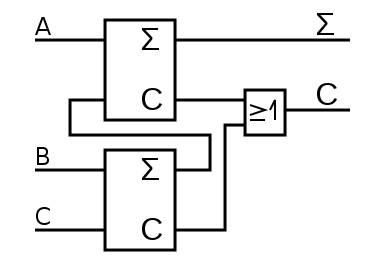
\includegraphics[scale=0.3]{full_adder.png}
	\caption{Full adder built of two half-adders.}
	\label{fig:full-adder}
\end{figure}
\begin{itemize}
	\item Fill in all possible combinations for $c_{in}$, $a$ and $b$ in table \ref{tab:full-adder-truth-table}. Think about what $\Sigma$ and $c_{out}$ should be and fill them in as well.
	\item Visually test the circuit drawing for all possible combinations and compare it with your expectations for $\Sigma$ and $c_{out}$. Do they match?

	\begin{table}[h]
		\centering
		\begin{tabular}{|c|c|c||c|c|}
			\hline
			$c_{in}$ & $a$ & $b$ & $\Sigma$ & $c_{out}$ \\ \hline
			&     &     &          &           \\ \hline
			&     &     &          &           \\ \hline
			&     &     &          &           \\ \hline
			&     &     &          &           \\ \hline
			&     &     &          &           \\ \hline
			&     &     &          &           \\ \hline
			&     &     &          &           \\ \hline
			&     &     &          &           \\ \hline
		\end{tabular}
		\caption{Truth table for the Full Adder.}
		\label{tab:full-adder-truth-table}
	\end{table}

	\item Once you have convinced yourself that the circuit is correct, translate it into only NAND gates by using the half-adders you derived earlier. (Hint: Do not transform the OR gate until the very end. You will see that it simpliefies very easily into a NAND gate.)
	\item Build the full adder on the breadboard.
\end{itemize}


\newpage